\newpage
\section{Diagramme d'États Comportementaux}\label{sec:diagramme_etatscomportementaux}
\begin{definition}[Diagramme d'\'Etats Comportementaux]
Un diagramme d'états comportementaux (Statechart) est un type de diagramme UML qui modélise des machines à états et présente une vue dynamique du système en mettant l'accent sur le comportment d'un objet ordonnancé par les événements.
\end{definition}

\begin{definition}[Action]
	Une action est une unité d’exécution automatique et non interruptible qui doit se terminer avant qu’une autre action puisse être considérée et ne peut pas être interrompue par une transition.
\end{definition}

\begin{definition}[Activité]
	Une activité est un ensemble d'actions ordonnées interne d'un état.
\end{definition}

\begin{definition}[Garde]
	Un garde (guard) est une condition qui doit être satisfaite pour que la transition ait lieu.
\end{definition}


\begin{table}[H]
	\centering
	\caption{Constitution d'un diagramme d'états comportementaux}
	\label{tbl:diagram_statechart_elements}
	\begin{adjustbox}{max width= \textwidth}
		\begin{tabular}{l|c}
			\toprule
			\textbf{\'El\'ement} & \textbf{Repr\'esentation}\\
			\midrule
			Diagramme d'\'etats & 
			\begin{minipage}{0.2\textwidth}
				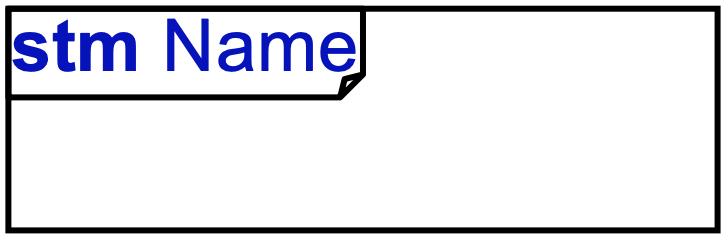
\includegraphics[scale=0.4]{./Images/Diagrammes/diagram_statechart_package.png}
			\end{minipage}\\
			\cmidrule(lr){1-2}
			\'Etat & 
			\begin{minipage}{0.2\textwidth}
				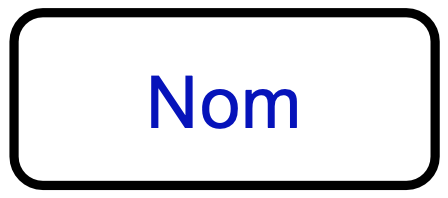
\includegraphics[scale=0.4]{./Images/Diagrammes/diagram_activite_elements_activite.png}
			\end{minipage}\\
			\cmidrule(lr){1-2}
			\'Etat initial  & 
			\begin{minipage}[l]{0.3\textwidth}
				\centering
				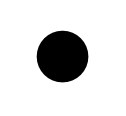
\includegraphics[scale=0.2]{./Images/Diagrammes/diagram_activite_elements_activite_initial.png}
			\end{minipage}\\
			\cmidrule(lr){1-2}
			\'Etat final & 
			\begin{minipage}[r]{0.3\textwidth}
				\centering
				
\includegraphics[scale=0.2]{./Images/Diagrammes/diagram_activite_elements_activite_final.png}
			\end{minipage}\\
			\cmidrule(lr){1-2}
			Transition d'\'etats & 
			\begin{minipage}{0.5\textwidth}
				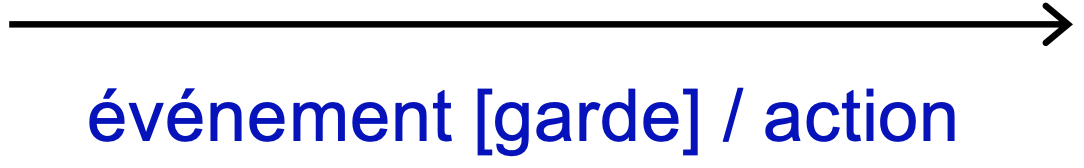
\includegraphics[width=\textwidth]{./Images/Diagrammes/diagram_statechart_transition.png}
				
			\end{minipage}\\
			\cmidrule(lr){1-2}
			Action de transition & 
			\begin{minipage}{0.5\textwidth}
				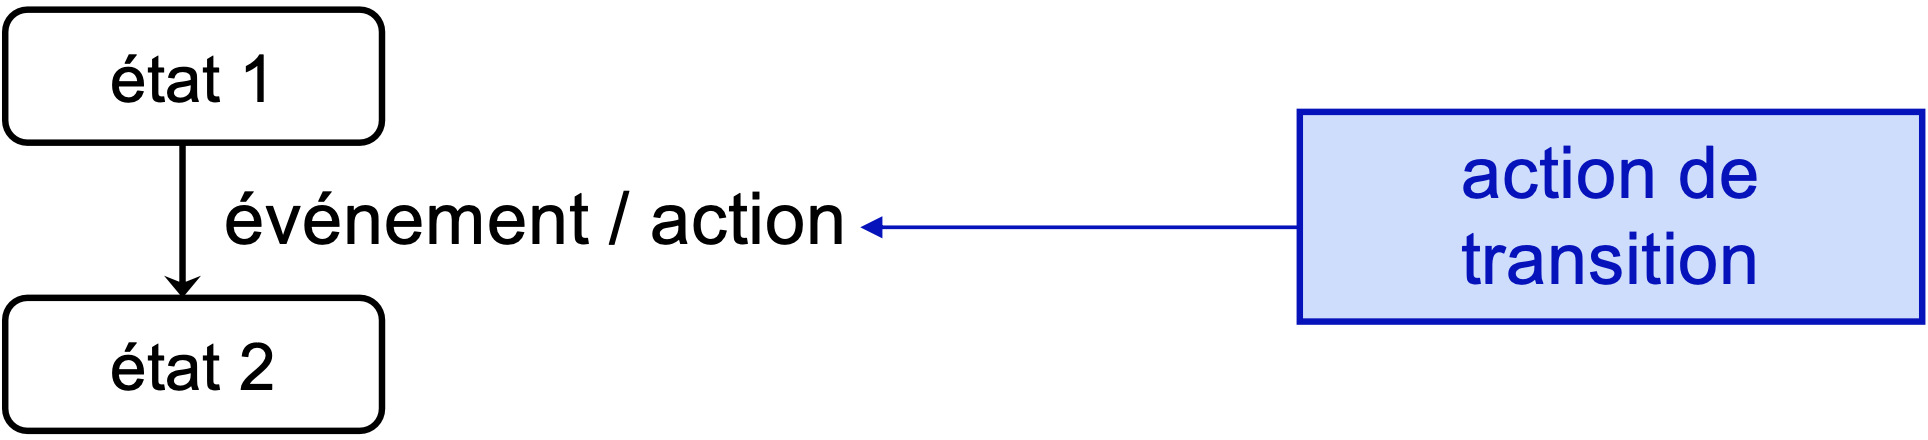
\includegraphics[width=\textwidth]{./Images/Diagrammes/diagram_statechart_actiontransition.png}
			\end{minipage}\\
			\cmidrule(lr){1-2}
			Activit\'e & 
			\begin{minipage}{0.5\textwidth}
				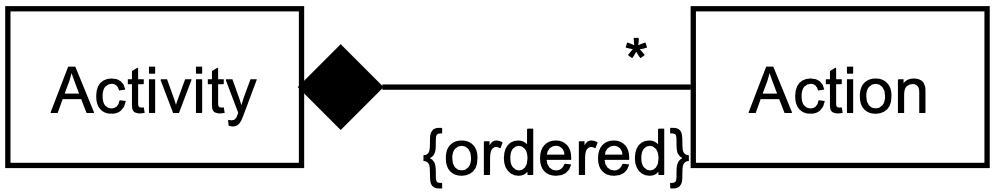
\includegraphics[width=\textwidth]{./Images/Diagrammes/diagram_statechart_activity_def.png}
			\end{minipage}\\
			\cmidrule(lr){1-2}
			\'Etat avec actions & 
			\begin{minipage}{0.5\textwidth}
				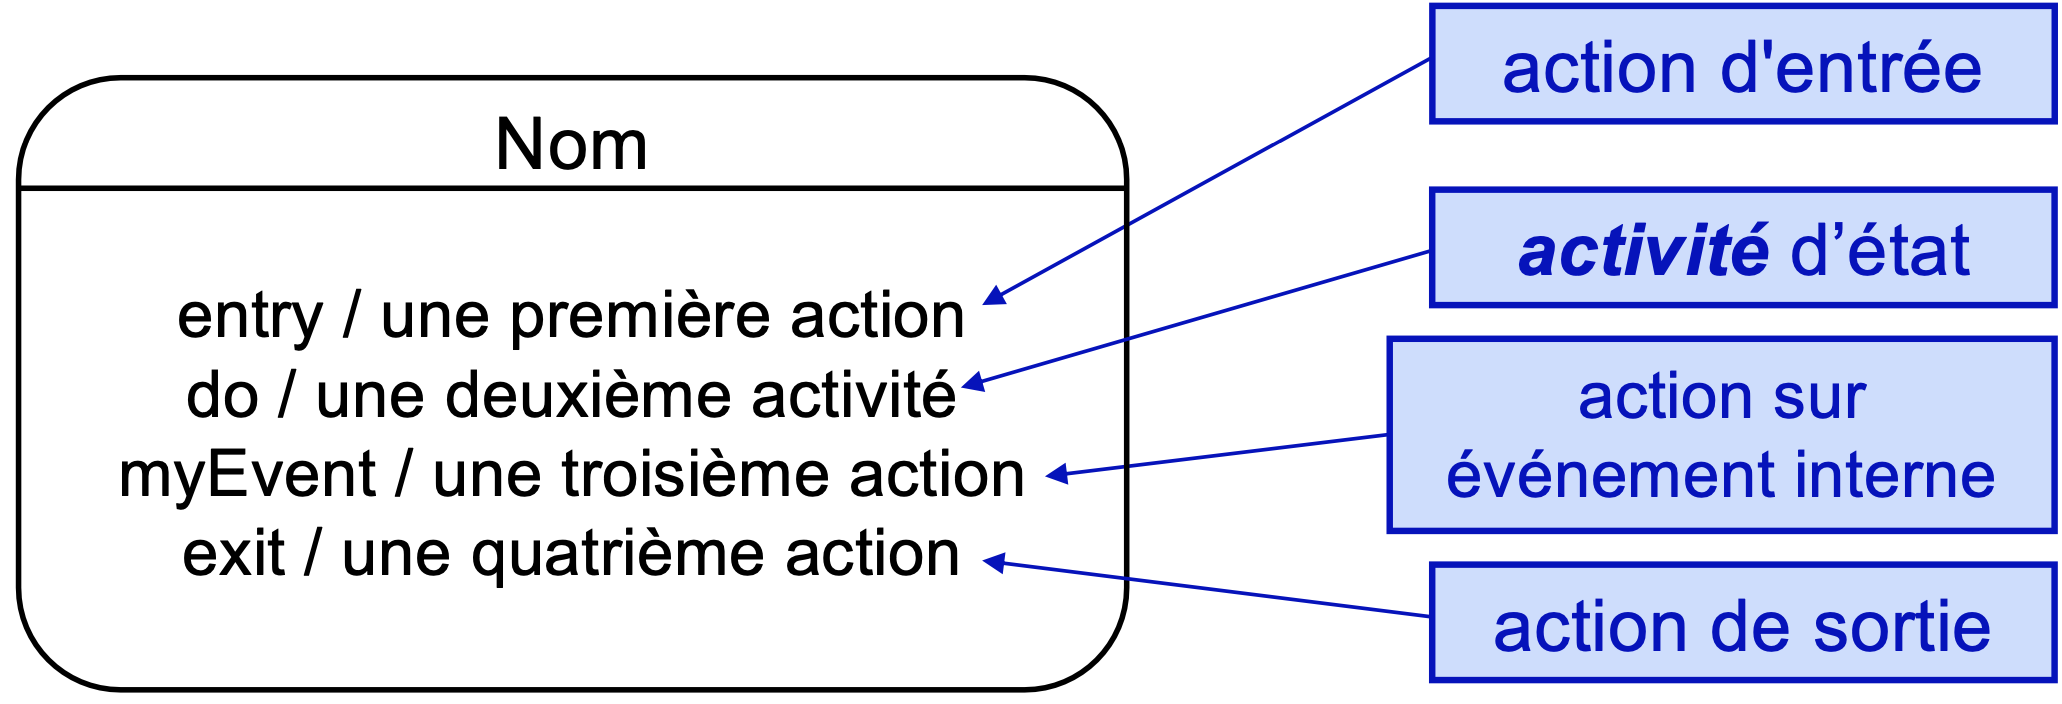
\includegraphics[width=\textwidth]{./Images/Diagrammes/diagram_statechart_etat_all.png}
				\tiny{Seules les activités associées à \og Do\fg sont interruptibles.}
			\end{minipage}\\
			\bottomrule
		\end{tabular}
	\end{adjustbox}
\end{table}







\begin{table}[H]
\caption{Types d'actions/activités}
\label{tbl:diagram_statechart_typesactions}
\begin{adjustbox}{max width=\textwidth}
\begin{tabular}{p{5em}|p{10em}|l|p{5em}}
\toprule
\textbf{Rapport à l'état}& \textbf{Type d'action} & \textbf{Déclenchement} & \textbf{Mot clé} \\
\midrule
Externe & Action de transition & Lorsqu'une transition est suivie &\\
\cmidrule(lr){1-4}
\multirow{5}{*}{Interne}& Action d'entrée & Lorsque le système entre dans un certain état & entry \\
\cmidrule(lr){2-4}
& Action de sortie & Lorsque le système sort d'un certain état & exit \\
\cmidrule(lr){2-4}
& Action temporelle & Se déclenche basée sur un événement temporel & every x s \\
\cmidrule(lr){2-4}
& Activité d'état & Se déroule tout le temps où l'on est dans l'état & do \\
\bottomrule
\end{tabular}
\end{adjustbox}
\end{table}

!!! Une activité peut être interrompue par une transition de sortie, car une activité est un esemble d'actions. Par contre, une action ne peut pas être interrompue.


\begin{figure}[H]
\centering
\begin{subfigure}{0.55\textwidth}
  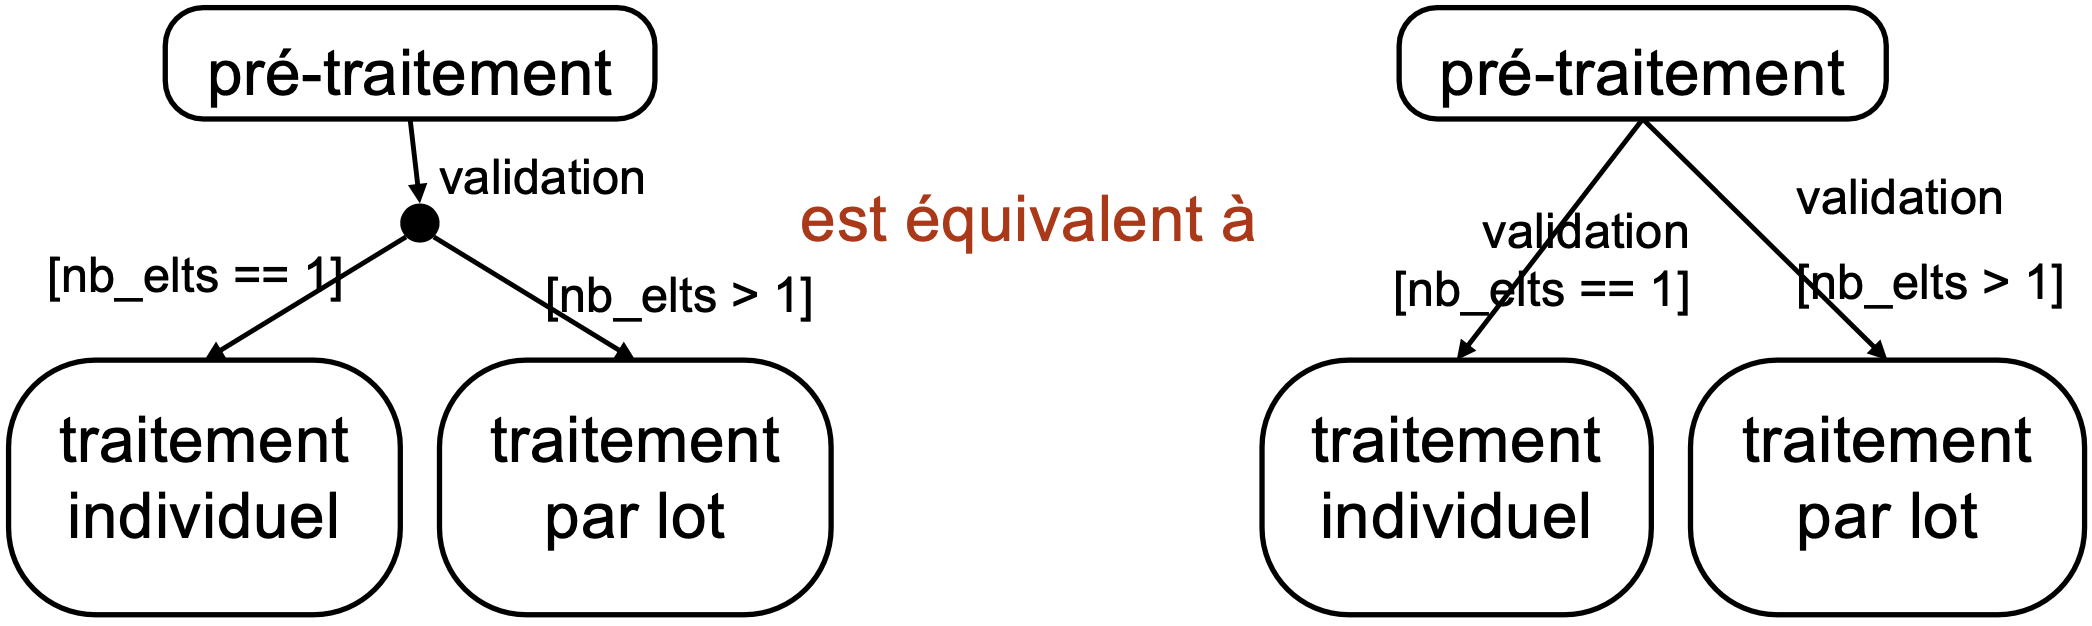
\includegraphics[width=\textwidth]{./Images/Diagrammes/diagram_statechart_pointjonctionstatique.png}
  \caption{Point de jonction statique.}
  \label{fig:diagram_statechart_pointjonctionstatique}
\end{subfigure}
\begin{subfigure}{0.4\textwidth}
  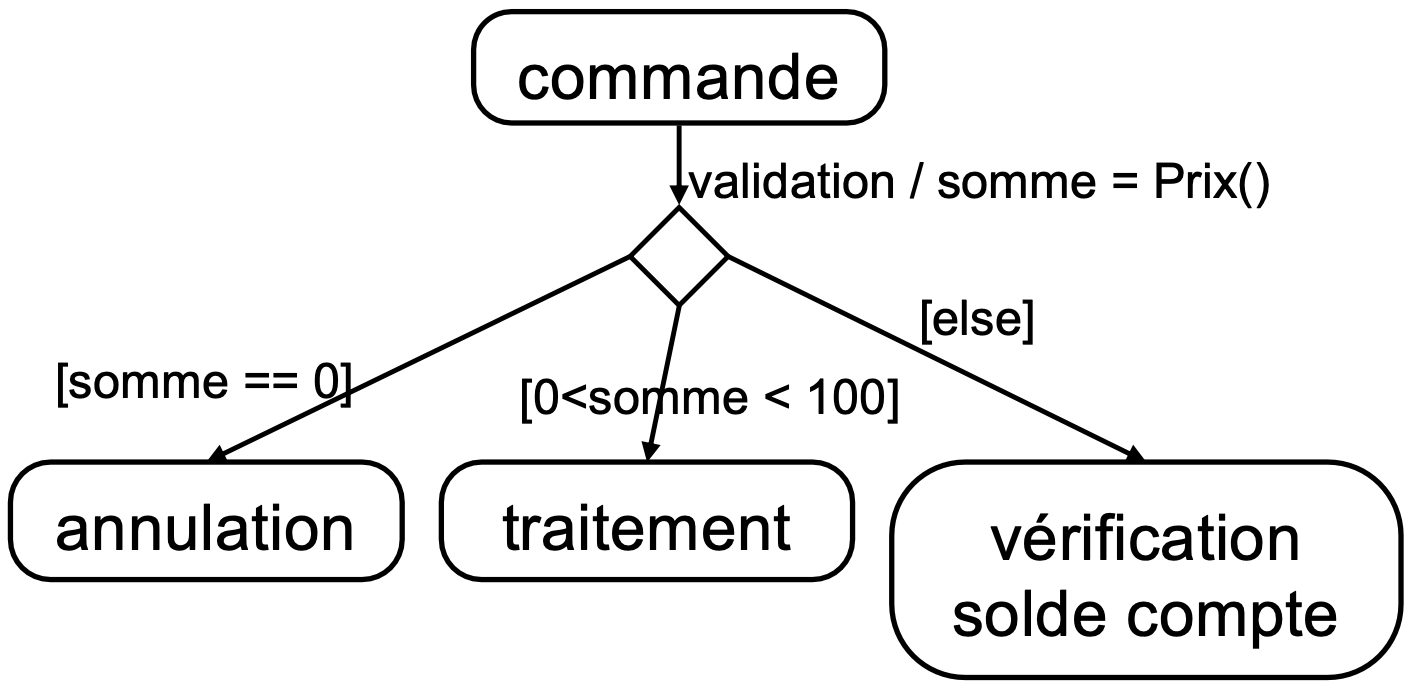
\includegraphics[width=\textwidth]{./Images/Diagrammes/diagram_statechart_pointjonctiondynamique.png}
  \caption{Point de jontion dynamique.}
  \label{fig:diagram_statechart_pointjonctiondynamique}
\end{subfigure}
\caption{Illustrations de Statecharts}
\label{fig:diagram_statechart_illustrations}
\end{figure}


\begin{figure}[H]
	\begin{subfigure}{0.5\textwidth}
		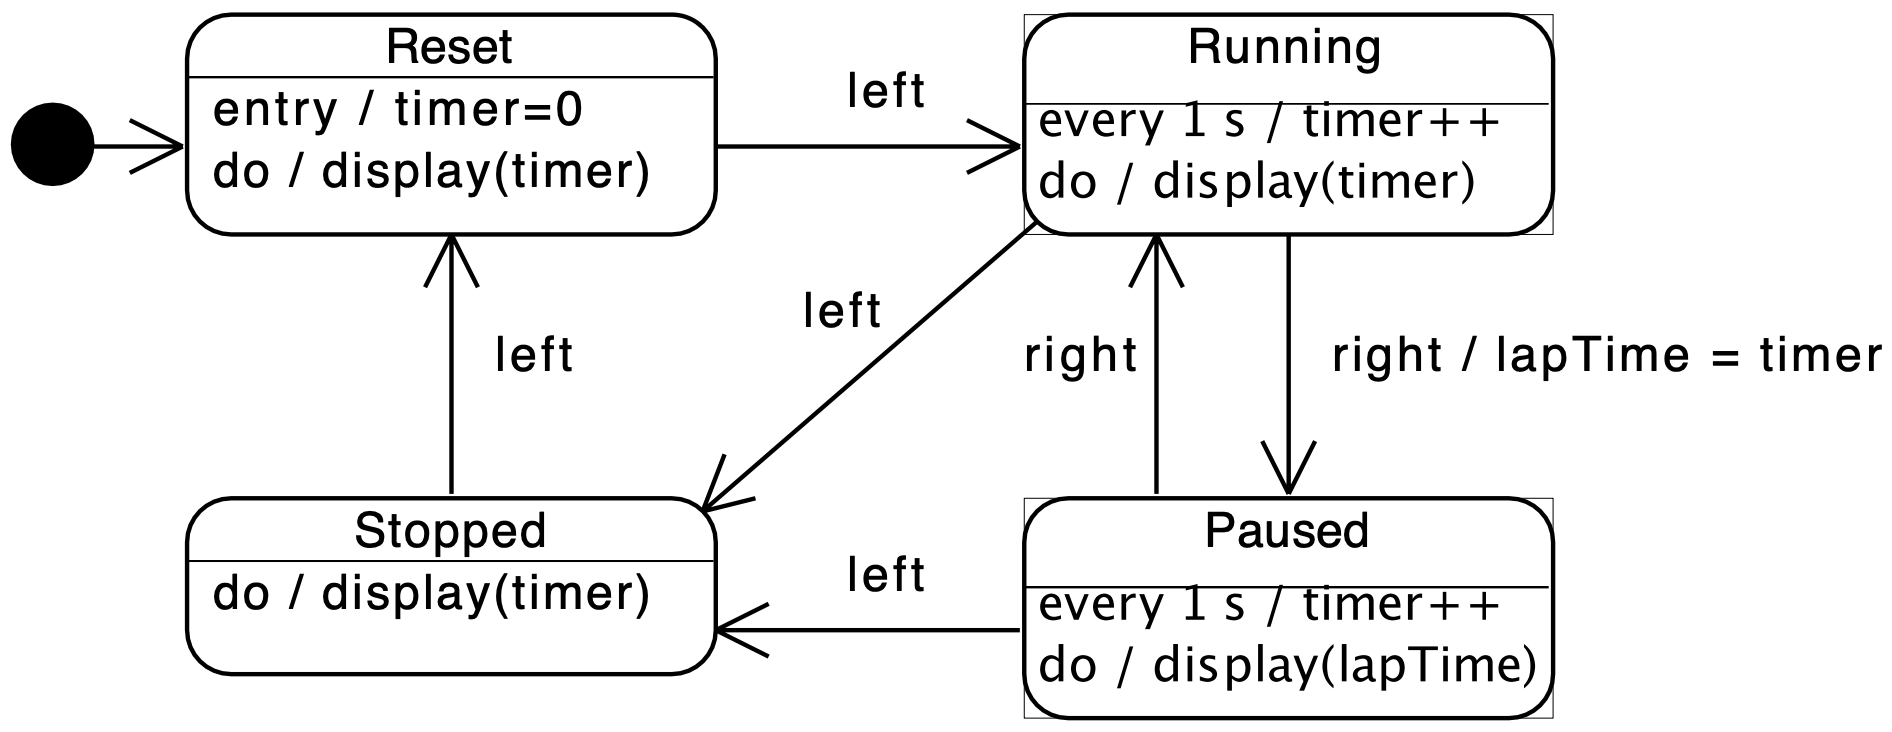
\includegraphics[width=\textwidth]{./Images/Diagrammes/diagram_statechart_ex_stopwatch_sansetatscomposites.png}
		\caption{Sans états composites.}
	\end{subfigure}
	\begin{subfigure}{0.5\textwidth}
		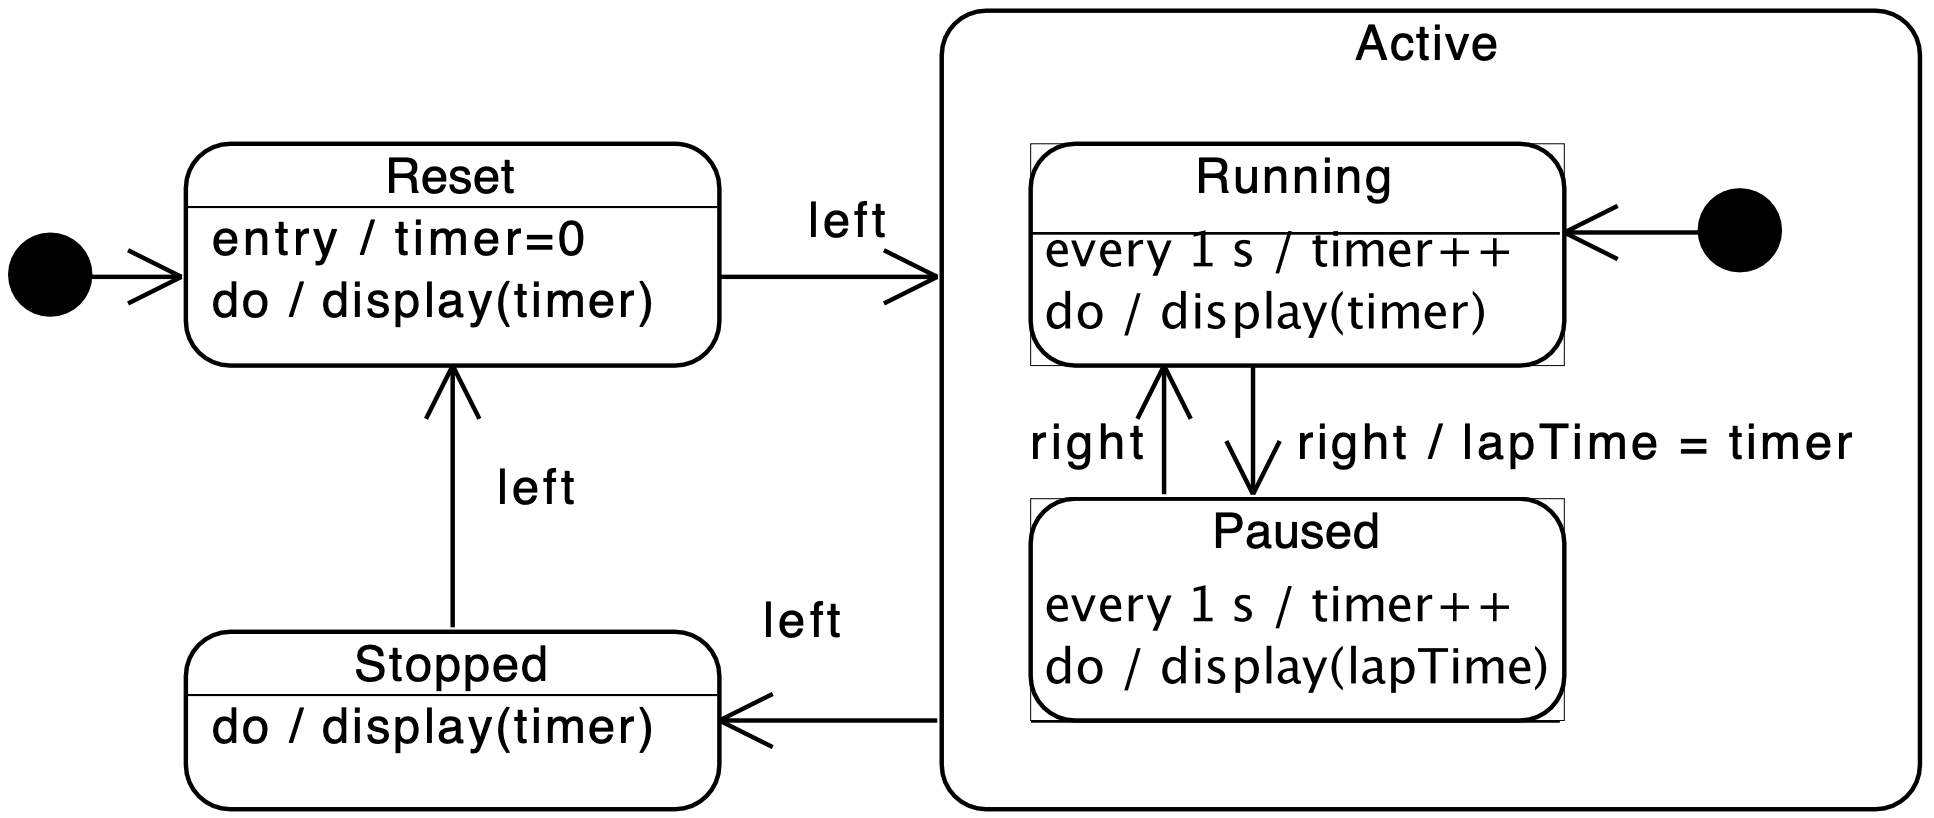
\includegraphics[width=\textwidth]{./Images/Diagrammes/diagram_statechart_ex_stopwatch_avecetatscomposites.png}
		\caption{Avec état de composition.}
	\end{subfigure}
	\caption{Exemple de Statechart : StopWatch}
\end{figure}